\documentclass{article}
\usepackage{mathtools}
\usepackage{amssymb}
\usepackage{amsthm}
\usepackage{physics}
\usepackage{stmaryrd}
\usepackage{bbm}
\usepackage{graphicx}
\usepackage{adjustbox}
\usepackage{hyperref}
\usepackage{tikz}
\usetikzlibrary{calc}
\usepackage{pgfplots}
\usepackage{minted}
\usepackage{subcaption}
\usepackage{algorithm}
\usepackage{algpseudocode}
\usepackage{graphicx}
\usepackage[margin=2cm]{geometry}
\hypersetup{
    colorlinks=true,
    linkcolor=blue,
    }
\usepackage{biblatex}
\addbibresource{refs.bib}
\usepackage{indentfirst}
\setlength{\parindent}{0.5cm}
\DeclareMathOperator{\Img}{Im}
\DeclareMathOperator{\Com}{Com}
\DeclareMathOperator{\End}{End}
\DeclareMathOperator{\Ker}{Ker}
\newtheorem{theorem}{Theoreme}
\newtheorem*{corollary}{Corollary}
\newtheorem{proposition}{Proposition}
\newtheorem{definition}{Definition}
\newtheorem{lemma}{Lemma}
\newtheorem{example}{Exemple}
\newtheorem{tactic}{Tactic}
\newcommand{\C}{\mathbb{C}}
\newcommand{\I}{\mathbb{I}}
\renewcommand{\L}{\mathcal{L}}
\newcommand{\Cn}{\mathscr{C}}
\renewcommand{\P}{\mathbb{P}}
\newcommand{\Z}{\mathbb{Z}}
\newcommand{\Q}{\mathbb{Q}}
\newcommand{\N}{\mathbb{N}}
\newcommand{\R}{\mathbb{R}}
\newcommand{\K}{\mathbb{K}}
\newcommand{\F}{\mathcal{F}}
\newcommand{\RM}[1]{\paragraph{RM} #1}
\DeclareMathOperator{\conv}{conv}
\DeclareMathOperator{\id}{id}

\begin{document}

\tableofcontents
\newpage
\setlength{\parskip}{7pt}
\section{Introduction - Motivation}

We were given several datasets from the website \textit{https://www.trictrac.net/} which sells a variety of board games. This website collects data for every article, such as reviews and grades posted by the users. 

Our task was to treat and analyze this data to try to gain information from it. One purpose was to classify these reviews and being able to predict the sentiment of review (positive or negative). 

This is a real-world application since the company could automatically gain insight on products by correlating words with grades.
The utilization of word vector representation and dimensionality reduction is useful in establishing meaningful associations between words and the sentiment expressed in reviews. The company could explore the represented space to find trends in what people like or dislike, and therefore potentially increasing sales.

\begin{figure}[H]
  \centering
  \begin{minipage}[t]{0.49\linewidth}
    \centering
    
\includegraphics[width=\linewidth]{tric_trac_pic.png}
    \caption{Tric Trac webpage}
  \end{minipage}\hfill
  \begin{minipage}[t]{0.49\linewidth}
    \centering
    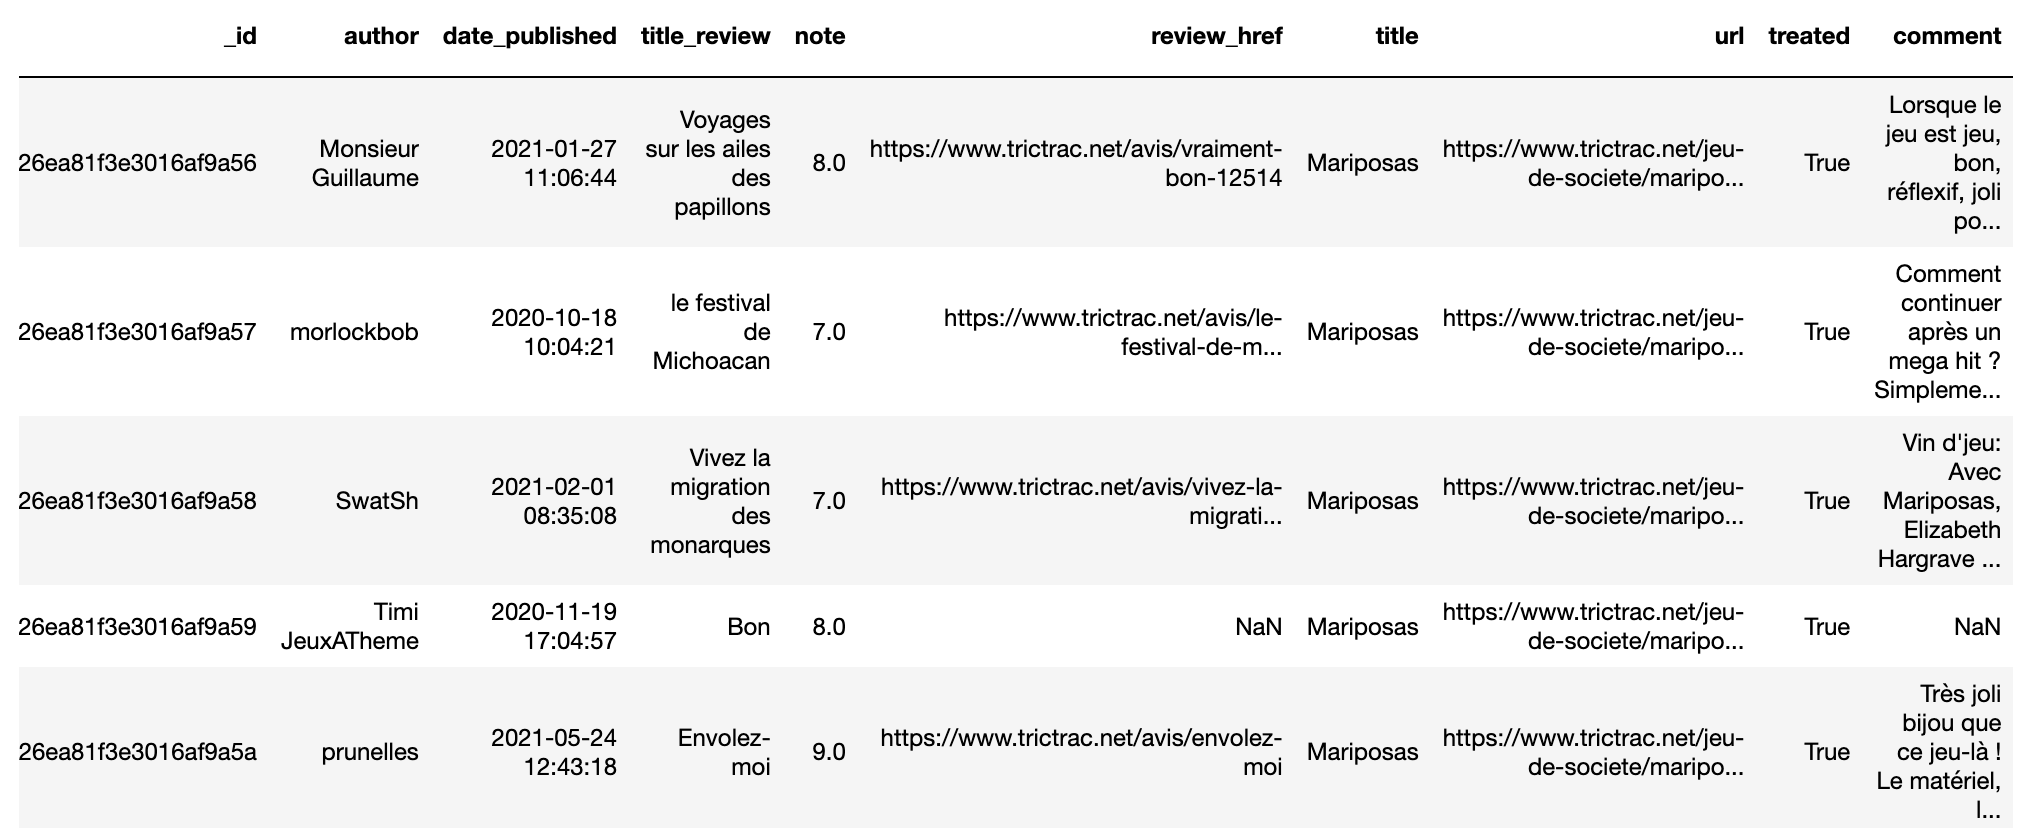
\includegraphics[width=\linewidth]{tric_trac_df.png}
    \caption{Tric Trac Dataframe}
  \end{minipage}
\end{figure}
The features X represent the \textit{comment} column and the target variable y is \textit{grade}.

So, what valuable insights can be extracted from these reviews? How can we effectively capture and quantify the sentiments conveyed?
The following report will highlight our methodology to uncover patterns, our data processing approaches and the potential of our findings.  
\newpage
\section{Descriptive statistics of the \textit{grades} feature}

We are starting by looking at the grades data, since it will be the criterion to classify reviews as positive or negative.
\begin{figure}[H]
  \centering
  \begin{minipage}[t]{0.49\linewidth}
    \centering
    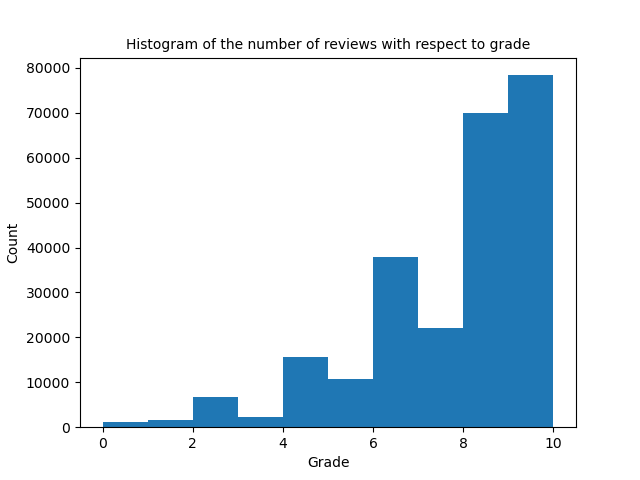
\includegraphics[width=\linewidth]{hist_plot_count.png}
  \end{minipage}\hfill
  \begin{minipage}[t]{0.49\linewidth}
    \centering
    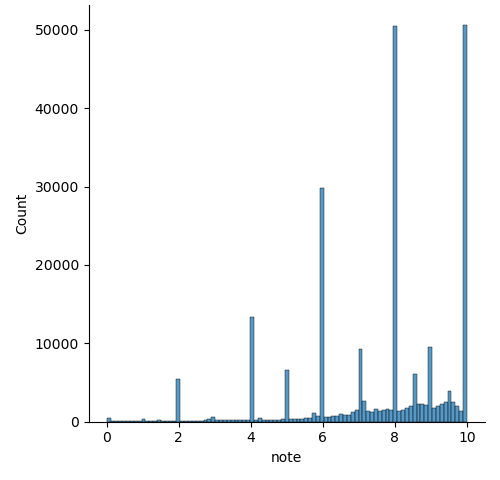
\includegraphics[width=\linewidth]{dist_plot_count.png}
  \end{minipage}
  \caption{Grade distribution}
\end{figure}

On the histogram on the left plot, 
we can notice that the majority of the grades are actually integers. Removing float numbers (or rounding to closest integer) could possibly simplify the model.
On the histogram plot , we can notice that the majority of reviews are actually positive.

It is cautious to already say it could introduce some challenges. Indeed, since grades are quite imbalanced, the model can become biased towards positive reviews. The model may tend to predict positive reviews more frequently, leading to lower accuracy for negative ones and an overall imbalance in predictions. Also, since there are fewer samples from negative reviews, the model may not have enough representative examples to learn the patterns and characteristics of the negative class.

\section{Text documents to vectors}

Text documents, in their raw form, consist of unstructured data that cannot be directly processed by machine learning algorithms. To effectively analyze and derive insights from text, it is necessary to transform the textual information into a numerical representation known as vectors because they provide a structured and quantifiable representation of textual information.

Therefore, since the features of the dataset represent the \textit{comment} feature, we will tackle ways to treat the data.
\subsection{Preprocessing}

Raw text data might contain unwanted or unimportant text due to which our results might not give efficient accuracy, and might make it hard to understand and analyze. So, proper pre-processing must be done on raw data.

We had to remove punctuation, URLs, numbers, accents, stopwords.
Stopwords are commonly used words in a language that are considered to have little or no significance in determining the meaning of a text.
`not' is not a stopword, because it might indicate the opposite sentiment.

We also applied Stemming that reduces words to their root forms. It minimizes the confusion around words that have similar meanings and lowers the complexity of the input space. However, it comes at the cost of throwing information away.

\subsection{One Hot Encoding}

One Hot Encoding is a vector representation of a word in vocabulary, ie the unique list of all the words appearing in the documents.
If the vocabulary size is n, each word in the vocabulary is therefore represented as a vector of size n. It takes binary values: 1 for the corresponding word and 0 otherwise.

\paragraph{On the implementation:}

We can represent the set of sentences as a tensor of shape (a, b, c) ie a matrices (number of sentences) of shape (b,c) where b represents the number of words in the sentence and c the vocabulary size.

\paragraph{Advantages:}

\begin{itemize}
  \item Intuitive and easy to implement
\end{itemize}

\paragraph{Inconvenients:}

\begin{itemize}
  \item Increase in dimensionality: a large vocabulary size implies a large number of columns, taking more memory size, which results in an increase in computational cost. + The matrix is sparse.
  \item Every vector sits in the orthogonal vector space so vectors are perpendicular to each other and are considered independent to each other, which is rarely the case.
  \item High chance of multi-collinearity due to dummy variables, which might affect the performance of the model (cf. Dummy Variable Trap)
\end{itemize}

\subsection{Bag of Words}

\subsection{tf-idf}

The BoW (Bag of Words) model assumes that the importance of a term is directly proportional to
the number of its appearance in the document, this can easily be misleading
when the most common words are `stopwords'. (But it really depends on
the algorithm that we are going to use afterwards, if we do perceptron, it wouldn't matter.)

But the BoW gives vectors with integer features, which may be favorable by some algorithm,
like Naive Bayes below. This being said, the tf-idf embedding gives vectors with features in $\mathbb{Q}$,
which can be dilated to integers.

tf-idf (term frequency - inverse document frequency) first considers
the whole of a corpus, it assumes a term too frequent in the corpus has little
information. Then it considers the importance of a term in a document
as the frequency of the term in this document times a scalar
representing its information in the corpus.

$$
\begin{aligned}
\mathrm{tfidf}(\mathrm{term}) & = \mathrm{tf}(\mathrm{term}) \times \mathrm{idf}(\mathrm{term}) \\
\mathrm{tf}(\mathrm{term}) & = \frac{\# \text { of times term appears in document }}{\# \text { of terms in document }} \\
\mathrm{idf}(\mathrm{term}) & =\ln \left(\frac{\# \text { of documents }}{\# \text { of documents in corpus with term }}\right)
\end{aligned}
$$

Other possible choices:

\begin{itemize}
  \item A term can be many (succesive) words (n-gram) (e.g. to
  take into account of negations before a word)
  \item The exact formulae can be changed while the same idea remains
\end{itemize}

\paragraph{On the implementation} Il faut éviter utiliser \verb|for|, et
utiliser les fonctions numpy à la place; on utilise les matrices sparse pour
gagner de la mémoire et parfois l'éfficacité.

\paragraph{Observations}
\begin{itemize}
  \item Curse of dimensionality
  \item Preprocessing is important
\end{itemize}

\section{Classification}

\subsection{Distances}

We can use euclidean distance, or we can use the distance concerning
only the angle between 2 vectors (so the `difference of lengths' of documents
is ignored).

$$
\begin{aligned}
&\text{(cosine similarity)}S(A, B) :=
\cos (\theta)=\frac{A \cdot B}{\|A\|\|B\|}\\
&\text{(cosine distance)}D(A, B) :=1-S(A, B)
\end{aligned}
$$

We see that cosine distance is better in nlp for 1. no curse of dimensionality; 2. no
need to reduce the dimension.

\subsection{Dimensionality reduction}

\begin{itemize}
  \item PCA (not useful for us, every new word (if not a stopword) can not be ignored and their linear combinations have no meaning)
  \item t-SNE (only useful for visualization?)
\end{itemize}

After the reduction of dimensionality, we may do a visulization; but
bad visulization results don't necessarily mean bad classification result.

\subsection{Naive Bayes}

The Naive Bayes algorithm do not require text representations such as one-hot encoding. It instead utilizes count vectorization to represent documents. Count vectorization preserves the word frequencies, allowing the algorithm to consider the importance of words in expressing sentiment.

Naive Bayes is a probabilistic classification algorithm.
It is called naive because it assumes that each input variable is independent.

We are looking for:

$$ \max_{y}\mathbb{P}(Y =y \mid X=(x_1, ..., x_n)) $$

using the Naive Bayes formula: $\mathbb{P}(Y \mid X) = \frac{\mathbb{P}(X\mid Y)\cdot \mathbb{P}(Y)}{\mathbb{P}(X)} = \frac{\mathbb{P}(Y)\prod_{i}^{}\mathbb{P}(X_i\mid Y)}{\mathbb{P}(X)}$
by independence,
where $\mathbb{P}(X\mid Y)$ is the likelihood, $\mathbb{P}(X)$ is the evidence, $\mathbb{P}(Y \mid X)$ is the posterior and $\mathbb{P}(Y)$ is the prior.

More precisely, we used Multinomial Naive Bayes for our task because it is suitable for discrete and count-based features, such as word frequencies in text data. The count vectorization of word aligns well with the assumptions of this model. It allows the model to estimate the probability of sentiment classes based on the frequency distribution of words.

\paragraph{Advantages} \begin{itemize}
\item Even though the independence assumption is rarely true, the model is still effective
\item Handles high dimensional data well
\end{itemize}

\paragraph{Inconvenients} \begin{itemize}
\item Estimated probability is often inaccurate because of the naive assumption
\end{itemize}

\subsection{K-Nearest neighbours}
\label{subset:KNN}

\paragraph{Algorithm} One predicts the information associated with a vector by the majority
of information associated with its neighbours (within k nearest).
We use tf-idf embedding here.
By simple experience
and raisonning (the length doesn't affect the positivity) as well, we chose cosine distance.

For comments of grades 4 - 7, they are more or less neutral, we can't
say if it is definitely positive or negative as human-being, so less chance
for our more or less naïve algorithm. For this reason we chose
to do our algorithm on comments of extremities.

We add a parameter to our algorithm: \textbf{balance}.
balance is a float >= 1 meaning that we trim the list of data of one label
of more quantity to size = balance$\times$(number of data with another label).
This is to solve the problem of disporpotional labelled data.

\paragraph{On the implementation} \begin{itemize}
  \item We favor the nearer information when there is a tie.
  \item Python is not a well typed language, it is so easy to have
  ridiculous bugs.
  \item Cosine distance works much better than euclidean distance.
  \item When the data is disporpotionally labelled, we need to balance the data to ensure performance for prediction of each label.
  \item We sometime use implemented fonctions to improve
  efficacity after having understood the method and
  implemented ourselves.
\end{itemize}

\paragraph{Positive} \begin{itemize}
  \item Easy to implement
\end{itemize}

\paragraph{Negative} \begin{itemize}
  \item Supervised
  \item $\Theta(n)$ for each prediction ($n$ the size of training data), which is
  very slow when we want to use a big training data to ensure better prediction.
\end{itemize}

\section{Evaluation of models - Results}

\subsection{Model evaluation}

First of all, the split the labeled dataset into training and testing subsets. The model is trained on the training data and then evaluated on the testing data to measure its performance, in order to assess its capacity to generalize predictions to unknown data.

Then, we used cross-validation for each model. It divides the data into parts, trains the model on some parts, and tests it on others. This process is repeated multiple times to get a reliable performance estimate. Cross-validation helps us understand how well the model works on unseen data and allows us to find the best settings for the model.

As mentioned earlier, the positive and negative classes are somehow imbalanced. Data stratification would be here inappropriate because the minority class will get underrepresented, since it has fewer samples.
Therefore, given the size of the dataset, an option would be to undersample the positive class: we train models with on data that has the same proportion of positive and negative classes.

Finally, the metrics we used are standard classification metrics such as precision, recall and F1 score.
Precision measures the accuracy of positive predictions. Recall measures the ability of the model to identify positive instances correctly. F1-score is a metric that combines precision and recall scores.

\paragraph{On implementation} We enable to specify random seed to ensure reproductivity.

\subsection{K-Nearest neighbors}

To begin with, we delibrately balanced the data, 50\% of positive comments (5000)
and 50\% of negative comments (5000).

By adjusting the $k$, we obtained such result shown in Figure~\ref{fig:KNN1}.

\begin{figure}[H]
  \centering
  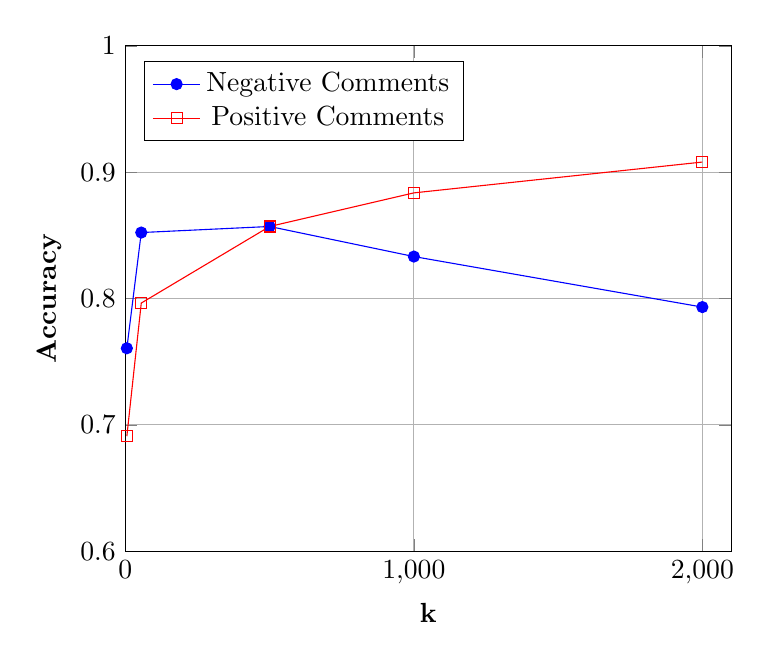
\begin{tikzpicture}
      \begin{axis}[
          xlabel={\textbf{k}},
          ylabel={\textbf{Accuracy}},
          xmin=0, xmax=2100,
          ymin=0.6, ymax=1,
          xtick={0,1000,2000,3000,4000,5000},
          ytick={0.6,0.7,0.8,0.9,1},
          legend pos=north west,
          grid=both,
          grid style={line width=0.2pt, draw=gray!30},
          major grid style={line width=0.4pt,draw=gray!60},
          height=8cm,
      ]
      \addplot[color=blue, mark=*] coordinates {
          (5,0.7606)
          (55,0.8522)
          (500,0.857)
          (1000,0.8332)
          (2000,0.7932)
      };
      \addplot[color=red, mark=square] coordinates {
          (5,0.691)
          (55,0.7964)
          (500,0.857)
          (1000,0.8836)
          (2000,0.908)
      };
      \legend{Negative Comments, Positive Comments}
      \end{axis}
  \end{tikzpicture}
  \caption{k nearest neighbor on balanced data}
  \label{fig:KNN1}
\end{figure}

That was some good results. But in the reality, our data is extremely disporpotional,
if we apply KNN directly, the algorithm would predict positive almost everytime. (Although
a positive comment has less chance to enter the neighbourhood of a negtive comment,
there are too many of them.) Indeed, we tried and get 0.26 as accuracy for negative comments and 0.94 for
positive comments.

The accuracy in total (on the data set) was good but it was not what we are after. We would like
$(r_p+r_n)/2$ to be big (so in the previous case it was 0.6). $r_{p/n}$ is the accuracy on the positive/negative comments.

To solve this problem, we use our \textbf{balance} parameter introduced before.

As the Figure~\ref{fig:balancenk} shows, the balance value would
better stay at 1 (otherwise it damages significantly
the accuracy on the negatives) and we increase k to
remedy the disadvantage of positive prediction.

Where does this disadvantage come from, while the number
of positives and negatives are equal in the training data (after trimming).
A conjecture of mine is that, the number of positive comments in the test data
is significantly less than that of the training data so
some vocabularies are not present in the training data. In this case,
we can only judge by more basic words and rely on bigger survey, thus increasing k helps.

\begin{figure}[H]
  \centering
  \begin{subfigure}[t]{0.33\textwidth}
    \centering
    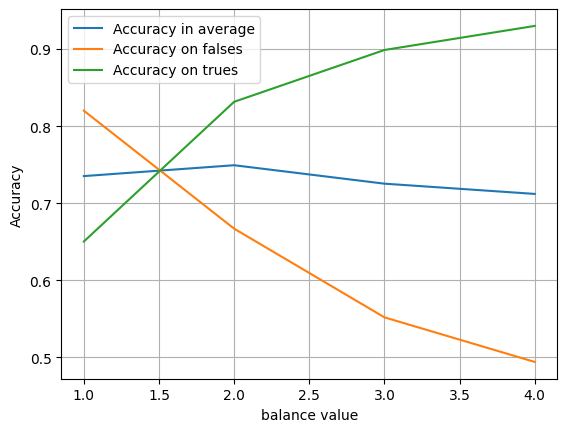
\includegraphics[width=\linewidth]{balancek5.png}
    \caption{k=5}
  \end{subfigure}%
  \hfill
  \begin{subfigure}[t]{0.33\textwidth}
    \centering
    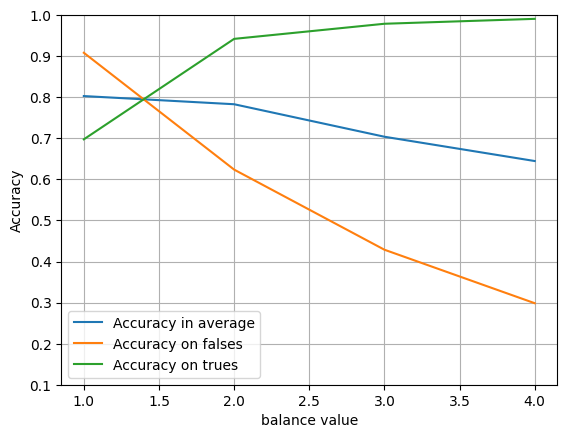
\includegraphics[width=\linewidth]{balancek50.png}
    \caption{k=50}
  \end{subfigure}
  \hfill
  \begin{subfigure}[t]{0.33\textwidth}
    \centering
    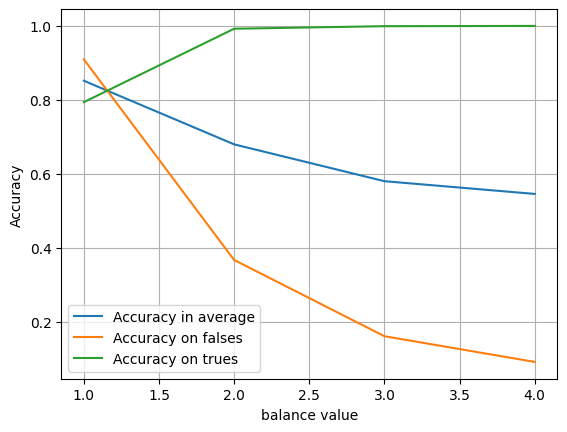
\includegraphics[width=\linewidth]{balancek500.png}
    \caption{k=500}
  \end{subfigure}
  \caption{Positive comments are labelled as true and negative comments are labelled as false}
  \label{fig:balancenk}
\end{figure}

Now we show a case in reality, our assumption/scenario is that :

The given data on the games is disproportional. Most comments are
positive. So positive comments do not give much information.
The manager then wants to detect then inspect all the negative comments
among all the comments.

Our KNN (with parameters balance=1, k=500 as explained in \ref{subset:KNN}) does this job.
So as shown in Table~\ref{tab:KNN}, we almost covered all negative comments,
the payoff is that the precision of class false is low, meaning
that the manager needs to see as much as 5 comments to read a true negative
comment.

\begin{table}[h]
  \centering
  \begin{tabular}{ccccc}
  \hline
  Class & Precision & Recall & F1-Score & Support \\
  \hline
  False & 0.73 & 0.28 & 0.41 & 6801 \\
  True & 0.89 & 0.98 & 0.93 & 39941 \\
  \hline
  Macro Avg & 0.81 & 0.63 & 0.67 & 46742 \\
  Weighted Avg & 0.87 & 0.88 & 0.86 & 46742 \\
  \hline
  \multicolumn{5}{c}{Accuracy = 0.88} \\
  \hline
  \end{tabular}
  \caption{Classification report with no undersampling}
  \label{tab:KNN}
\end{table}

\subsection{Naive Bayes}

\begin{table}[H]
  \centering
  \begin{tabular}{ccccc}
  \hline
  Class & Precision & Recall & F1-Score & Support \\
  \hline
  False & 0.73 & 0.28 & 0.41 & 6801 \\
  True & 0.89 & 0.98 & 0.93 & 39941 \\
  \hline
  Macro Avg & 0.81 & 0.63 & 0.67 & 46742 \\
  Weighted Avg & 0.87 & 0.88 & 0.86 & 46742 \\
  \hline
  \multicolumn{5}{c}{Accuracy = 0.88} \\
  \hline
  \end{tabular}
  \caption{Classification report with no undersampling}
  \label{tab:KNN}
\end{table}

\begin{table}[H]
  \centering
  \begin{tabular}{ccccc}
  \hline
  Class & Precision & Recall & F1-Score & Support \\
  \hline
  0.0 & 0.86 & 0.84 & 0.85 & 6781 \\
  1.0 & 0.84 & 0.86 & 0.85 & 6721 \\
  \hline
  Macro Avg & 0.85 & 0.85 & 0.85 & 13502 \\
  Weighted Avg & 0.85 & 0.85 & 0.85 & 13502 \\
  \hline
  \multicolumn{5}{c}{Accuracy = 0.85} \\
  \hline
  \end{tabular}
  \caption{Classification report with undersampling}
  \label{tab:classification_report}
\end{table}

We notice that without undersampling, the F1 score is very high for the positive class but it is low for the negative. The model is biased towards predicting positive sentiment, leading to a higher number of false negatives. 
However, with undersampling, the F1-score is lower for the positive class but it as at least balanced with the negative class. This situation is certainly favorable. 

We are diving into the training phase with looking at learning curves. This is giving us an idea on how well the model generalizes to testing data.

\begin{figure}[H]
  \centering
  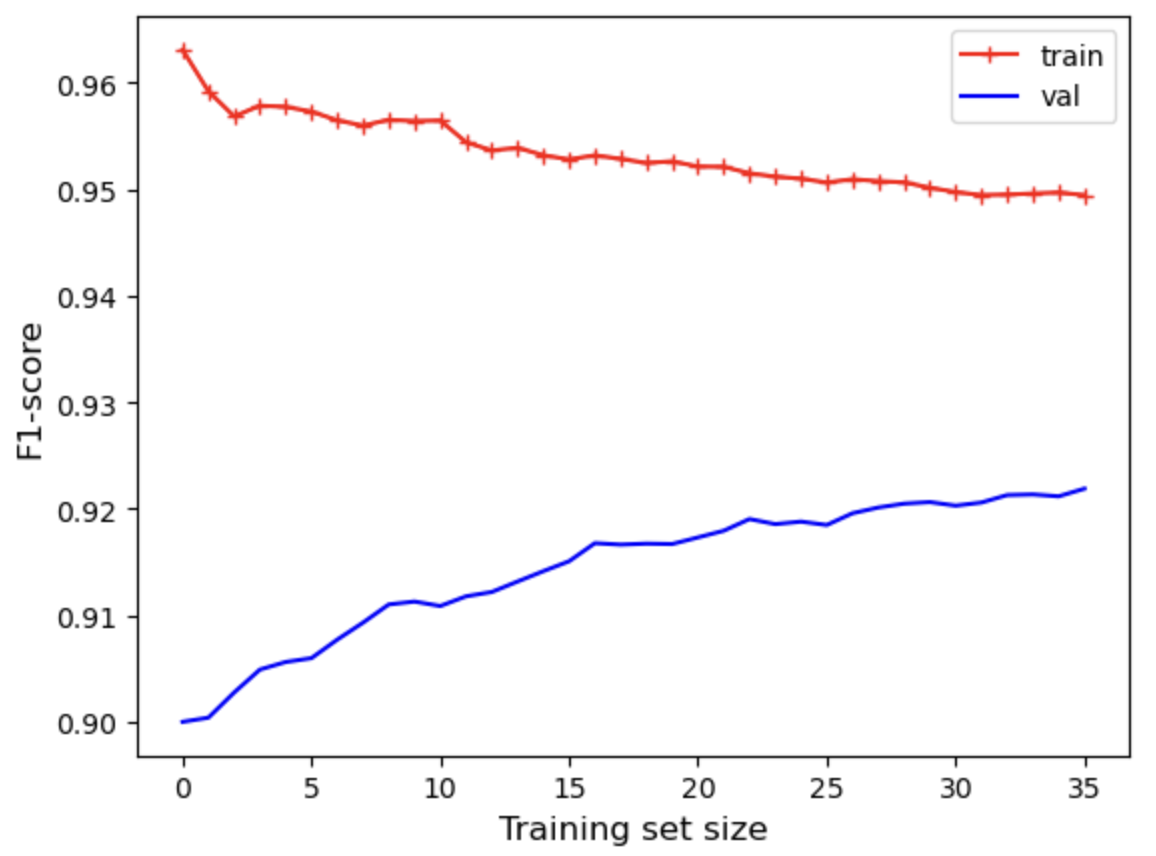
\includegraphics[height=7cm]{nb_start_learning_curves.png}
  \caption{Learning curves for Multinomial NB with undersampling (with training size in thousands)}
  \label{fig:image_label}
\end{figure}

We can see that the training F1-score is a bit larger than the testing F1-score, which was expected since the model training is done on the training set. Still, the difference still is small so it is going well. 

\section{Insights - Analysis}

\subsection{Challenges encountered}

The most challenging task was to process data since the dataset is very large. We realized how efficient libraries are, since their computation time is low compared to when we implement it all by hand.
The implementations are optimized, and the computations are designed for performance. Moreover, libraries such as the ones from sklearn take advantage of parallel computing (executed on multi-core processors). 

Another challenge encountered is that it was not obvious at first how to apply preprocessing. Indeed, we had to think about how much we wanted to remove stopwords or common words. Removing these words might simplify the model, but we might also lose information with it. Another example is the use of negative contractions. It was not obvious if they could have a significant impact or not.

A common obstacle with NLP is that sentences are far from being perfect, even after preprocessing is applied. Sentiment classifiers can also struggle when encountering words or phrases that were not present in the training data, so that's why using word embeddings are useful to generalize to unknown terms. 

\subsection{Lessons learned throughout the project}

The importance of preprocessing is a first lesson we could remember from this project. Indeed, without preprocessing, making a mathematical representation of words does not make any sense since the word embedding space will have a very large dimension, thus making predictions almost impossible.

Then, handling class imbalance. It is easy to classify reviews as positive when the majority of reviews in the training data are positive. Undersampling was a good solution to this problem (no it's not..). 

\subsection{Limitations and areas of improvement}

Sentiment is subjective, and annotating large datasets with sentiment labels can be challenging due to varying interpretations. Consequently, different customers might assign different sentiment scores, leading to inconsistencies in the training and evaluation data. Additionally, sentiment analysis can be dependent on the context, making it challenging to capture the nuances and sarcasm present in text. 

Another challenge is the domain adaptation problem, because our model is trained on one domain and may struggle to generalize well to other domains due to differences in language usage and sentiment expressions.

We could evaluate the ability of our model to generalize to reviews from other fields (such as movies reviews) and see if it can transfer its knowledge pretty well or not.

Finally, the models we used to represent text data were not sequential for the most part, instead it focused on the words themselves. An option would be to use Deep Learning models such as recurrent neural networks (RNNs), long short-term memory (LSTM) networks, or transformer-based architectures (e.g., BERT, GPT). These models can capture complex linguistic patterns and contextual information. 

\section{Topological data analysis, persistent homology}

In this section we introduce a method for analysing a text
without a parameter (e.g.\ k in KNN), in fact, we consider all
the possibility of parameters. Moreover, we want to be able to
find a meaningful correspondence between the computation and
the text. We use persistent homology.

But for this matter, for simplicity and the reason of capacity
of the author, we have to change our task.

This is a project report instead of a course note, so the importance
is not on the details of the algorithm but rather the ideas and experiments.
But the algorithm and the theory in themselves are interesting and not
easy to be found clearly on the internet, so for the clearness of the report
we include concisely the necessary
concepts and key algorithms there \ref{theoretical}.

\subsection{Essay grading}

Inherently, persistent homology is useful when it comes to 3d modeling.
But in data analysis in general, it is also useful (e.g.\ analyse the
performance of a basketball team and get a intuitive view of the team structure).

Here we use the persistent homology to analyse essays and grading.

Roughly speaking, a better discoursive essay should have a
richer writting structure, (a proposition should be discussed
in different angles, the last paragraph echos to the beginning etc.).
Translated in persistent homology,
if a good essay is a topological space, it should have
many holes (homology groups). For example,
in Figure~\ref{apple}, the essay have a statement, and then some arguments,
, finally a conclusion. 1 - 2 - 3 - 4 are linked by time order, 1 - 4 are linked because they are similar.
This hole means good argument. There are also filled triangles (2-simplices), those
sentences form clusters, so they are filled instead of forming holes.
(We are going to introduce how to build concretely simplicial complexes very soon.)

\begin{figure}[H]
  \centering
  

\tikzset{every picture/.style={line width=0.75pt}} %set default line width to 0.75pt        

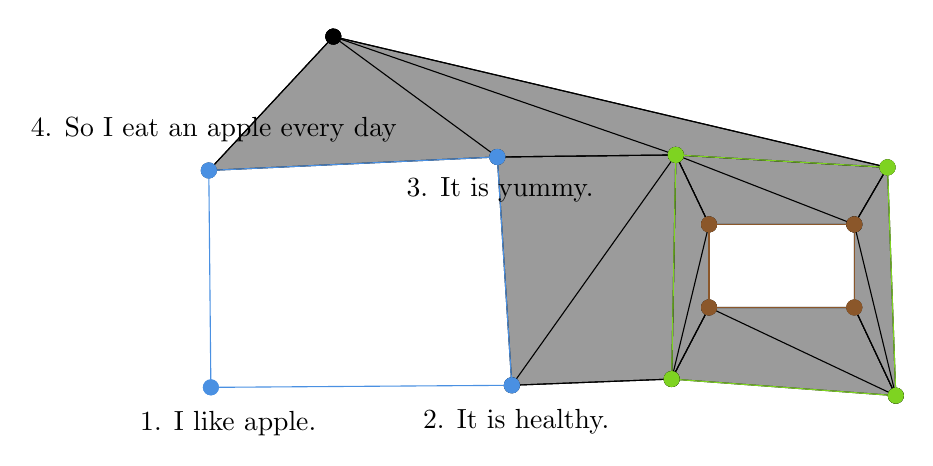
\begin{tikzpicture}[x=0.75pt,y=0.75pt,yscale=-1,xscale=1]
%uncomment if require: \path (0,300); %set diagram left start at 0, and has height of 300

%Shape: Polygon [id:ds506045927728886] 
\draw  [fill={rgb, 255:red, 155; green, 155; blue, 155 }  ,fill opacity=1 ] (337,211.5) -- (355,177) -- (425,177) -- (445,219.5) -- cycle ;
%Shape: Polygon [id:ds373063136182463] 
\draw  [fill={rgb, 255:red, 155; green, 155; blue, 155 }  ,fill opacity=1 ] (441,109.5) -- (425,137) -- (355,137) -- (339,103.5) -- cycle ;
%Shape: Polygon [id:ds04357467087348055] 
\draw  [fill={rgb, 255:red, 155; green, 155; blue, 155 }  ,fill opacity=1 ] (445,219.5) -- (425,177) -- (425,137) -- (441,109.5) -- cycle ;
%Shape: Polygon [id:ds8597694080078087] 
\draw  [fill={rgb, 255:red, 155; green, 155; blue, 155 }  ,fill opacity=1 ] (339,103.5) -- (355,137) -- (355,177) -- (337,211.5) -- cycle ;

%Straight Lines [id:da7958699538877538] 
\draw    (339,103.5) -- (425,137) ;
\draw [shift={(425,137)}, rotate = 21.28] [color={rgb, 255:red, 0; green, 0; blue, 0 }  ][fill={rgb, 255:red, 0; green, 0; blue, 0 }  ][line width=0.75]      (0, 0) circle [x radius= 3.35, y radius= 3.35]   ;
\draw [shift={(339,103.5)}, rotate = 21.28] [color={rgb, 255:red, 0; green, 0; blue, 0 }  ][fill={rgb, 255:red, 0; green, 0; blue, 0 }  ][line width=0.75]      (0, 0) circle [x radius= 3.35, y radius= 3.35]   ;
%Straight Lines [id:da37382810612047734] 
\draw    (425,137) -- (445,219.5) ;
\draw [shift={(445,219.5)}, rotate = 76.37] [color={rgb, 255:red, 0; green, 0; blue, 0 }  ][fill={rgb, 255:red, 0; green, 0; blue, 0 }  ][line width=0.75]      (0, 0) circle [x radius= 3.35, y radius= 3.35]   ;
\draw [shift={(425,137)}, rotate = 76.37] [color={rgb, 255:red, 0; green, 0; blue, 0 }  ][fill={rgb, 255:red, 0; green, 0; blue, 0 }  ][line width=0.75]      (0, 0) circle [x radius= 3.35, y radius= 3.35]   ;
%Straight Lines [id:da33578118329024775] 
\draw    (355,177) -- (445,219.5) ;
\draw [shift={(445,219.5)}, rotate = 25.28] [color={rgb, 255:red, 0; green, 0; blue, 0 }  ][fill={rgb, 255:red, 0; green, 0; blue, 0 }  ][line width=0.75]      (0, 0) circle [x radius= 3.35, y radius= 3.35]   ;
\draw [shift={(355,177)}, rotate = 25.28] [color={rgb, 255:red, 0; green, 0; blue, 0 }  ][fill={rgb, 255:red, 0; green, 0; blue, 0 }  ][line width=0.75]      (0, 0) circle [x radius= 3.35, y radius= 3.35]   ;
%Straight Lines [id:da27555178758587107] 
\draw    (355,137) -- (337,211.5) ;
\draw [shift={(337,211.5)}, rotate = 103.58] [color={rgb, 255:red, 0; green, 0; blue, 0 }  ][fill={rgb, 255:red, 0; green, 0; blue, 0 }  ][line width=0.75]      (0, 0) circle [x radius= 3.35, y radius= 3.35]   ;
\draw [shift={(355,137)}, rotate = 103.58] [color={rgb, 255:red, 0; green, 0; blue, 0 }  ][fill={rgb, 255:red, 0; green, 0; blue, 0 }  ][line width=0.75]      (0, 0) circle [x radius= 3.35, y radius= 3.35]   ;
%Shape: Polygon [id:ds20124875657376728] 
\draw  [fill={rgb, 255:red, 155; green, 155; blue, 155 }  ,fill opacity=1 ] (253,104.5) -- (260,214.5) -- (337,211.5) -- (339,103.5) -- cycle ;
%Shape: Polygon [id:ds3619467537546437] 
\draw  [fill={rgb, 255:red, 155; green, 155; blue, 155 }  ,fill opacity=1 ] (174,46.5) -- (441,109.5) -- (339,103.5) -- (253,104.5) -- (114,111) -- cycle ;
%Straight Lines [id:da5963075508320128] 
\draw    (339,103.5) -- (253,104.5) ;
\draw [shift={(253,104.5)}, rotate = 179.33] [color={rgb, 255:red, 0; green, 0; blue, 0 }  ][fill={rgb, 255:red, 0; green, 0; blue, 0 }  ][line width=0.75]      (0, 0) circle [x radius= 3.35, y radius= 3.35]   ;
\draw [shift={(339,103.5)}, rotate = 179.33] [color={rgb, 255:red, 0; green, 0; blue, 0 }  ][fill={rgb, 255:red, 0; green, 0; blue, 0 }  ][line width=0.75]      (0, 0) circle [x radius= 3.35, y radius= 3.35]   ;
%Straight Lines [id:da8612090103920278] 
\draw    (260,214.5) -- (339,103.5) ;
\draw [shift={(339,103.5)}, rotate = 305.44] [color={rgb, 255:red, 0; green, 0; blue, 0 }  ][fill={rgb, 255:red, 0; green, 0; blue, 0 }  ][line width=0.75]      (0, 0) circle [x radius= 3.35, y radius= 3.35]   ;
\draw [shift={(260,214.5)}, rotate = 305.44] [color={rgb, 255:red, 0; green, 0; blue, 0 }  ][fill={rgb, 255:red, 0; green, 0; blue, 0 }  ][line width=0.75]      (0, 0) circle [x radius= 3.35, y radius= 3.35]   ;
%Straight Lines [id:da9692653745827828] 
\draw    (260,214.5) -- (337,211.5) ;
\draw [shift={(337,211.5)}, rotate = 357.77] [color={rgb, 255:red, 0; green, 0; blue, 0 }  ][fill={rgb, 255:red, 0; green, 0; blue, 0 }  ][line width=0.75]      (0, 0) circle [x radius= 3.35, y radius= 3.35]   ;
\draw [shift={(260,214.5)}, rotate = 357.77] [color={rgb, 255:red, 0; green, 0; blue, 0 }  ][fill={rgb, 255:red, 0; green, 0; blue, 0 }  ][line width=0.75]      (0, 0) circle [x radius= 3.35, y radius= 3.35]   ;
%Straight Lines [id:da7164877740446134] 
\draw    (114,111) -- (174,46.5) ;
\draw [shift={(174,46.5)}, rotate = 312.93] [color={rgb, 255:red, 0; green, 0; blue, 0 }  ][fill={rgb, 255:red, 0; green, 0; blue, 0 }  ][line width=0.75]      (0, 0) circle [x radius= 3.35, y radius= 3.35]   ;
\draw [shift={(114,111)}, rotate = 312.93] [color={rgb, 255:red, 0; green, 0; blue, 0 }  ][fill={rgb, 255:red, 0; green, 0; blue, 0 }  ][line width=0.75]      (0, 0) circle [x radius= 3.35, y radius= 3.35]   ;
%Straight Lines [id:da2125405974487078] 
\draw    (174,46.5) -- (253,104.5) ;
\draw [shift={(253,104.5)}, rotate = 36.29] [color={rgb, 255:red, 0; green, 0; blue, 0 }  ][fill={rgb, 255:red, 0; green, 0; blue, 0 }  ][line width=0.75]      (0, 0) circle [x radius= 3.35, y radius= 3.35]   ;
\draw [shift={(174,46.5)}, rotate = 36.29] [color={rgb, 255:red, 0; green, 0; blue, 0 }  ][fill={rgb, 255:red, 0; green, 0; blue, 0 }  ][line width=0.75]      (0, 0) circle [x radius= 3.35, y radius= 3.35]   ;
%Straight Lines [id:da8884288301278187] 
\draw    (174,46.5) -- (441,109.5) ;
\draw [shift={(441,109.5)}, rotate = 13.28] [color={rgb, 255:red, 0; green, 0; blue, 0 }  ][fill={rgb, 255:red, 0; green, 0; blue, 0 }  ][line width=0.75]      (0, 0) circle [x radius= 3.35, y radius= 3.35]   ;
\draw [shift={(174,46.5)}, rotate = 13.28] [color={rgb, 255:red, 0; green, 0; blue, 0 }  ][fill={rgb, 255:red, 0; green, 0; blue, 0 }  ][line width=0.75]      (0, 0) circle [x radius= 3.35, y radius= 3.35]   ;
%Straight Lines [id:da3878057357434834] 
\draw    (174,46.5) -- (339,103.5) ;
\draw [shift={(339,103.5)}, rotate = 19.06] [color={rgb, 255:red, 0; green, 0; blue, 0 }  ][fill={rgb, 255:red, 0; green, 0; blue, 0 }  ][line width=0.75]      (0, 0) circle [x radius= 3.35, y radius= 3.35]   ;
\draw [shift={(174,46.5)}, rotate = 19.06] [color={rgb, 255:red, 0; green, 0; blue, 0 }  ][fill={rgb, 255:red, 0; green, 0; blue, 0 }  ][line width=0.75]      (0, 0) circle [x radius= 3.35, y radius= 3.35]   ;
%Straight Lines [id:da3895078416872] 
\draw [color={rgb, 255:red, 126; green, 211; blue, 33 }  ,draw opacity=1 ]   (445,219.5) -- (337,211.5) ;
\draw [shift={(337,211.5)}, rotate = 184.24] [color={rgb, 255:red, 126; green, 211; blue, 33 }  ,draw opacity=1 ][fill={rgb, 255:red, 126; green, 211; blue, 33 }  ,fill opacity=1 ][line width=0.75]      (0, 0) circle [x radius= 3.35, y radius= 3.35]   ;
\draw [shift={(445,219.5)}, rotate = 184.24] [color={rgb, 255:red, 126; green, 211; blue, 33 }  ,draw opacity=1 ][fill={rgb, 255:red, 126; green, 211; blue, 33 }  ,fill opacity=1 ][line width=0.75]      (0, 0) circle [x radius= 3.35, y radius= 3.35]   ;
%Straight Lines [id:da300892222460144] 
\draw [color={rgb, 255:red, 74; green, 144; blue, 226 }  ,draw opacity=1 ]   (114,111) -- (115,215.5) ;
\draw [shift={(115,215.5)}, rotate = 89.45] [color={rgb, 255:red, 74; green, 144; blue, 226 }  ,draw opacity=1 ][fill={rgb, 255:red, 74; green, 144; blue, 226 }  ,fill opacity=1 ][line width=0.75]      (0, 0) circle [x radius= 3.35, y radius= 3.35]   ;
\draw [shift={(114,111)}, rotate = 89.45] [color={rgb, 255:red, 74; green, 144; blue, 226 }  ,draw opacity=1 ][fill={rgb, 255:red, 74; green, 144; blue, 226 }  ,fill opacity=1 ][line width=0.75]      (0, 0) circle [x radius= 3.35, y radius= 3.35]   ;
%Straight Lines [id:da5712067967796253] 
\draw [color={rgb, 255:red, 74; green, 144; blue, 226 }  ,draw opacity=1 ]   (115,215.5) -- (260,214.5) ;
\draw [shift={(260,214.5)}, rotate = 359.6] [color={rgb, 255:red, 74; green, 144; blue, 226 }  ,draw opacity=1 ][fill={rgb, 255:red, 74; green, 144; blue, 226 }  ,fill opacity=1 ][line width=0.75]      (0, 0) circle [x radius= 3.35, y radius= 3.35]   ;
\draw [shift={(115,215.5)}, rotate = 359.6] [color={rgb, 255:red, 74; green, 144; blue, 226 }  ,draw opacity=1 ][fill={rgb, 255:red, 74; green, 144; blue, 226 }  ,fill opacity=1 ][line width=0.75]      (0, 0) circle [x radius= 3.35, y radius= 3.35]   ;
%Straight Lines [id:da998130260097339] 
\draw [color={rgb, 255:red, 74; green, 144; blue, 226 }  ,draw opacity=1 ]   (260,214.5) -- (253,104.5) ;
\draw [shift={(253,104.5)}, rotate = 266.36] [color={rgb, 255:red, 74; green, 144; blue, 226 }  ,draw opacity=1 ][fill={rgb, 255:red, 74; green, 144; blue, 226 }  ,fill opacity=1 ][line width=0.75]      (0, 0) circle [x radius= 3.35, y radius= 3.35]   ;
\draw [shift={(260,214.5)}, rotate = 266.36] [color={rgb, 255:red, 74; green, 144; blue, 226 }  ,draw opacity=1 ][fill={rgb, 255:red, 74; green, 144; blue, 226 }  ,fill opacity=1 ][line width=0.75]      (0, 0) circle [x radius= 3.35, y radius= 3.35]   ;
%Straight Lines [id:da15833915226992357] 
\draw [color={rgb, 255:red, 74; green, 144; blue, 226 }  ,draw opacity=1 ]   (114,111) -- (253,104.5) ;
\draw [shift={(253,104.5)}, rotate = 357.32] [color={rgb, 255:red, 74; green, 144; blue, 226 }  ,draw opacity=1 ][fill={rgb, 255:red, 74; green, 144; blue, 226 }  ,fill opacity=1 ][line width=0.75]      (0, 0) circle [x radius= 3.35, y radius= 3.35]   ;
\draw [shift={(114,111)}, rotate = 357.32] [color={rgb, 255:red, 74; green, 144; blue, 226 }  ,draw opacity=1 ][fill={rgb, 255:red, 74; green, 144; blue, 226 }  ,fill opacity=1 ][line width=0.75]      (0, 0) circle [x radius= 3.35, y radius= 3.35]   ;
%Straight Lines [id:da1551244874188762] 
\draw    (441,109.5) -- (425,137) ;
\draw [shift={(425,137)}, rotate = 120.19] [color={rgb, 255:red, 0; green, 0; blue, 0 }  ][fill={rgb, 255:red, 0; green, 0; blue, 0 }  ][line width=0.75]      (0, 0) circle [x radius= 3.35, y radius= 3.35]   ;
\draw [shift={(441,109.5)}, rotate = 120.19] [color={rgb, 255:red, 0; green, 0; blue, 0 }  ][fill={rgb, 255:red, 0; green, 0; blue, 0 }  ][line width=0.75]      (0, 0) circle [x radius= 3.35, y radius= 3.35]   ;
%Straight Lines [id:da45803051915893067] 
\draw    (425,177) -- (445,219.5) ;
\draw [shift={(445,219.5)}, rotate = 64.8] [color={rgb, 255:red, 0; green, 0; blue, 0 }  ][fill={rgb, 255:red, 0; green, 0; blue, 0 }  ][line width=0.75]      (0, 0) circle [x radius= 3.35, y radius= 3.35]   ;
\draw [shift={(425,177)}, rotate = 64.8] [color={rgb, 255:red, 0; green, 0; blue, 0 }  ][fill={rgb, 255:red, 0; green, 0; blue, 0 }  ][line width=0.75]      (0, 0) circle [x radius= 3.35, y radius= 3.35]   ;
%Straight Lines [id:da3656558768012268] 
\draw    (355,177) -- (337,211.5) ;
\draw [shift={(337,211.5)}, rotate = 117.55] [color={rgb, 255:red, 0; green, 0; blue, 0 }  ][fill={rgb, 255:red, 0; green, 0; blue, 0 }  ][line width=0.75]      (0, 0) circle [x radius= 3.35, y radius= 3.35]   ;
\draw [shift={(355,177)}, rotate = 117.55] [color={rgb, 255:red, 0; green, 0; blue, 0 }  ][fill={rgb, 255:red, 0; green, 0; blue, 0 }  ][line width=0.75]      (0, 0) circle [x radius= 3.35, y radius= 3.35]   ;
%Straight Lines [id:da6696032151723832] 
\draw    (355,137) -- (339,103.5) ;
\draw [shift={(339,103.5)}, rotate = 244.47] [color={rgb, 255:red, 0; green, 0; blue, 0 }  ][fill={rgb, 255:red, 0; green, 0; blue, 0 }  ][line width=0.75]      (0, 0) circle [x radius= 3.35, y radius= 3.35]   ;
\draw [shift={(355,137)}, rotate = 244.47] [color={rgb, 255:red, 0; green, 0; blue, 0 }  ][fill={rgb, 255:red, 0; green, 0; blue, 0 }  ][line width=0.75]      (0, 0) circle [x radius= 3.35, y radius= 3.35]   ;
%Straight Lines [id:da9412473128467516] 
\draw [color={rgb, 255:red, 126; green, 211; blue, 33 }  ,draw opacity=1 ]   (337,211.5) -- (339,103.5) ;
\draw [shift={(339,103.5)}, rotate = 271.06] [color={rgb, 255:red, 126; green, 211; blue, 33 }  ,draw opacity=1 ][fill={rgb, 255:red, 126; green, 211; blue, 33 }  ,fill opacity=1 ][line width=0.75]      (0, 0) circle [x radius= 3.35, y radius= 3.35]   ;
\draw [shift={(337,211.5)}, rotate = 271.06] [color={rgb, 255:red, 126; green, 211; blue, 33 }  ,draw opacity=1 ][fill={rgb, 255:red, 126; green, 211; blue, 33 }  ,fill opacity=1 ][line width=0.75]      (0, 0) circle [x radius= 3.35, y radius= 3.35]   ;
%Straight Lines [id:da40626776597378655] 
\draw [color={rgb, 255:red, 126; green, 211; blue, 33 }  ,draw opacity=1 ]   (441,109.5) -- (445,219.5) ;
\draw [shift={(445,219.5)}, rotate = 87.92] [color={rgb, 255:red, 126; green, 211; blue, 33 }  ,draw opacity=1 ][fill={rgb, 255:red, 126; green, 211; blue, 33 }  ,fill opacity=1 ][line width=0.75]      (0, 0) circle [x radius= 3.35, y radius= 3.35]   ;
\draw [shift={(441,109.5)}, rotate = 87.92] [color={rgb, 255:red, 126; green, 211; blue, 33 }  ,draw opacity=1 ][fill={rgb, 255:red, 126; green, 211; blue, 33 }  ,fill opacity=1 ][line width=0.75]      (0, 0) circle [x radius= 3.35, y radius= 3.35]   ;
%Straight Lines [id:da39887955488152826] 
\draw [color={rgb, 255:red, 126; green, 211; blue, 33 }  ,draw opacity=1 ]   (441,109.5) -- (339,103.5) ;
\draw [shift={(339,103.5)}, rotate = 183.37] [color={rgb, 255:red, 126; green, 211; blue, 33 }  ,draw opacity=1 ][fill={rgb, 255:red, 126; green, 211; blue, 33 }  ,fill opacity=1 ][line width=0.75]      (0, 0) circle [x radius= 3.35, y radius= 3.35]   ;
\draw [shift={(441,109.5)}, rotate = 183.37] [color={rgb, 255:red, 126; green, 211; blue, 33 }  ,draw opacity=1 ][fill={rgb, 255:red, 126; green, 211; blue, 33 }  ,fill opacity=1 ][line width=0.75]      (0, 0) circle [x radius= 3.35, y radius= 3.35]   ;
%Straight Lines [id:da42956969917858223] 
\draw [color={rgb, 255:red, 139; green, 87; blue, 42 }  ,draw opacity=1 ]   (425,137) -- (355,137) ;
\draw [shift={(355,137)}, rotate = 180] [color={rgb, 255:red, 139; green, 87; blue, 42 }  ,draw opacity=1 ][fill={rgb, 255:red, 139; green, 87; blue, 42 }  ,fill opacity=1 ][line width=0.75]      (0, 0) circle [x radius= 3.35, y radius= 3.35]   ;
\draw [shift={(425,137)}, rotate = 180] [color={rgb, 255:red, 139; green, 87; blue, 42 }  ,draw opacity=1 ][fill={rgb, 255:red, 139; green, 87; blue, 42 }  ,fill opacity=1 ][line width=0.75]      (0, 0) circle [x radius= 3.35, y radius= 3.35]   ;
%Straight Lines [id:da14852397184426325] 
\draw [color={rgb, 255:red, 139; green, 87; blue, 42 }  ,draw opacity=1 ]   (425,177) -- (425,137) ;
\draw [shift={(425,137)}, rotate = 270] [color={rgb, 255:red, 139; green, 87; blue, 42 }  ,draw opacity=1 ][fill={rgb, 255:red, 139; green, 87; blue, 42 }  ,fill opacity=1 ][line width=0.75]      (0, 0) circle [x radius= 3.35, y radius= 3.35]   ;
\draw [shift={(425,177)}, rotate = 270] [color={rgb, 255:red, 139; green, 87; blue, 42 }  ,draw opacity=1 ][fill={rgb, 255:red, 139; green, 87; blue, 42 }  ,fill opacity=1 ][line width=0.75]      (0, 0) circle [x radius= 3.35, y radius= 3.35]   ;
%Straight Lines [id:da7173822720349425] 
\draw [color={rgb, 255:red, 139; green, 87; blue, 42 }  ,draw opacity=1 ]   (355,177) -- (425,177) ;
\draw [shift={(425,177)}, rotate = 0] [color={rgb, 255:red, 139; green, 87; blue, 42 }  ,draw opacity=1 ][fill={rgb, 255:red, 139; green, 87; blue, 42 }  ,fill opacity=1 ][line width=0.75]      (0, 0) circle [x radius= 3.35, y radius= 3.35]   ;
\draw [shift={(355,177)}, rotate = 0] [color={rgb, 255:red, 139; green, 87; blue, 42 }  ,draw opacity=1 ][fill={rgb, 255:red, 139; green, 87; blue, 42 }  ,fill opacity=1 ][line width=0.75]      (0, 0) circle [x radius= 3.35, y radius= 3.35]   ;
%Straight Lines [id:da6148683084406998] 
\draw [color={rgb, 255:red, 139; green, 87; blue, 42 }  ,draw opacity=1 ]   (355,177) -- (355,137) ;
\draw [shift={(355,137)}, rotate = 270] [color={rgb, 255:red, 139; green, 87; blue, 42 }  ,draw opacity=1 ][fill={rgb, 255:red, 139; green, 87; blue, 42 }  ,fill opacity=1 ][line width=0.75]      (0, 0) circle [x radius= 3.35, y radius= 3.35]   ;
\draw [shift={(355,177)}, rotate = 270] [color={rgb, 255:red, 139; green, 87; blue, 42 }  ,draw opacity=1 ][fill={rgb, 255:red, 139; green, 87; blue, 42 }  ,fill opacity=1 ][line width=0.75]      (0, 0) circle [x radius= 3.35, y radius= 3.35]   ;

% Text Node
\draw (79.67,225.67) node [anchor=north west][inner sep=0.75pt]   [align=left] {1. I like apple.};
% Text Node
\draw (216,225) node [anchor=north west][inner sep=0.75pt]   [align=left] {2. It is healthy.};
% Text Node
\draw (208,113) node [anchor=north west][inner sep=0.75pt]   [align=left] {3. It is yummy.};
% Text Node
\draw (27,84) node [anchor=north west][inner sep=0.75pt]   [align=left] {4. So I eat an apple every day};


\end{tikzpicture}
  \caption{There are 2 holes in this simplicial complex,
  one represented by the blue cycle and one by brown.
  Note that the brown cycle and the green cycle are homology equivalent, so they count as one.}
  \label{apple}
\end{figure}

If we only have one such graph, we will have to determine the similarity to link.
However, different similarity bars can give different simplicial complexes and have
different homology groups. Structure changes with scale, e.g.\ Figure~\ref{fig:scale}.
So our approache will consider all the scales (whence ``persistent'' homology).

\begin{figure}[H]
\centering
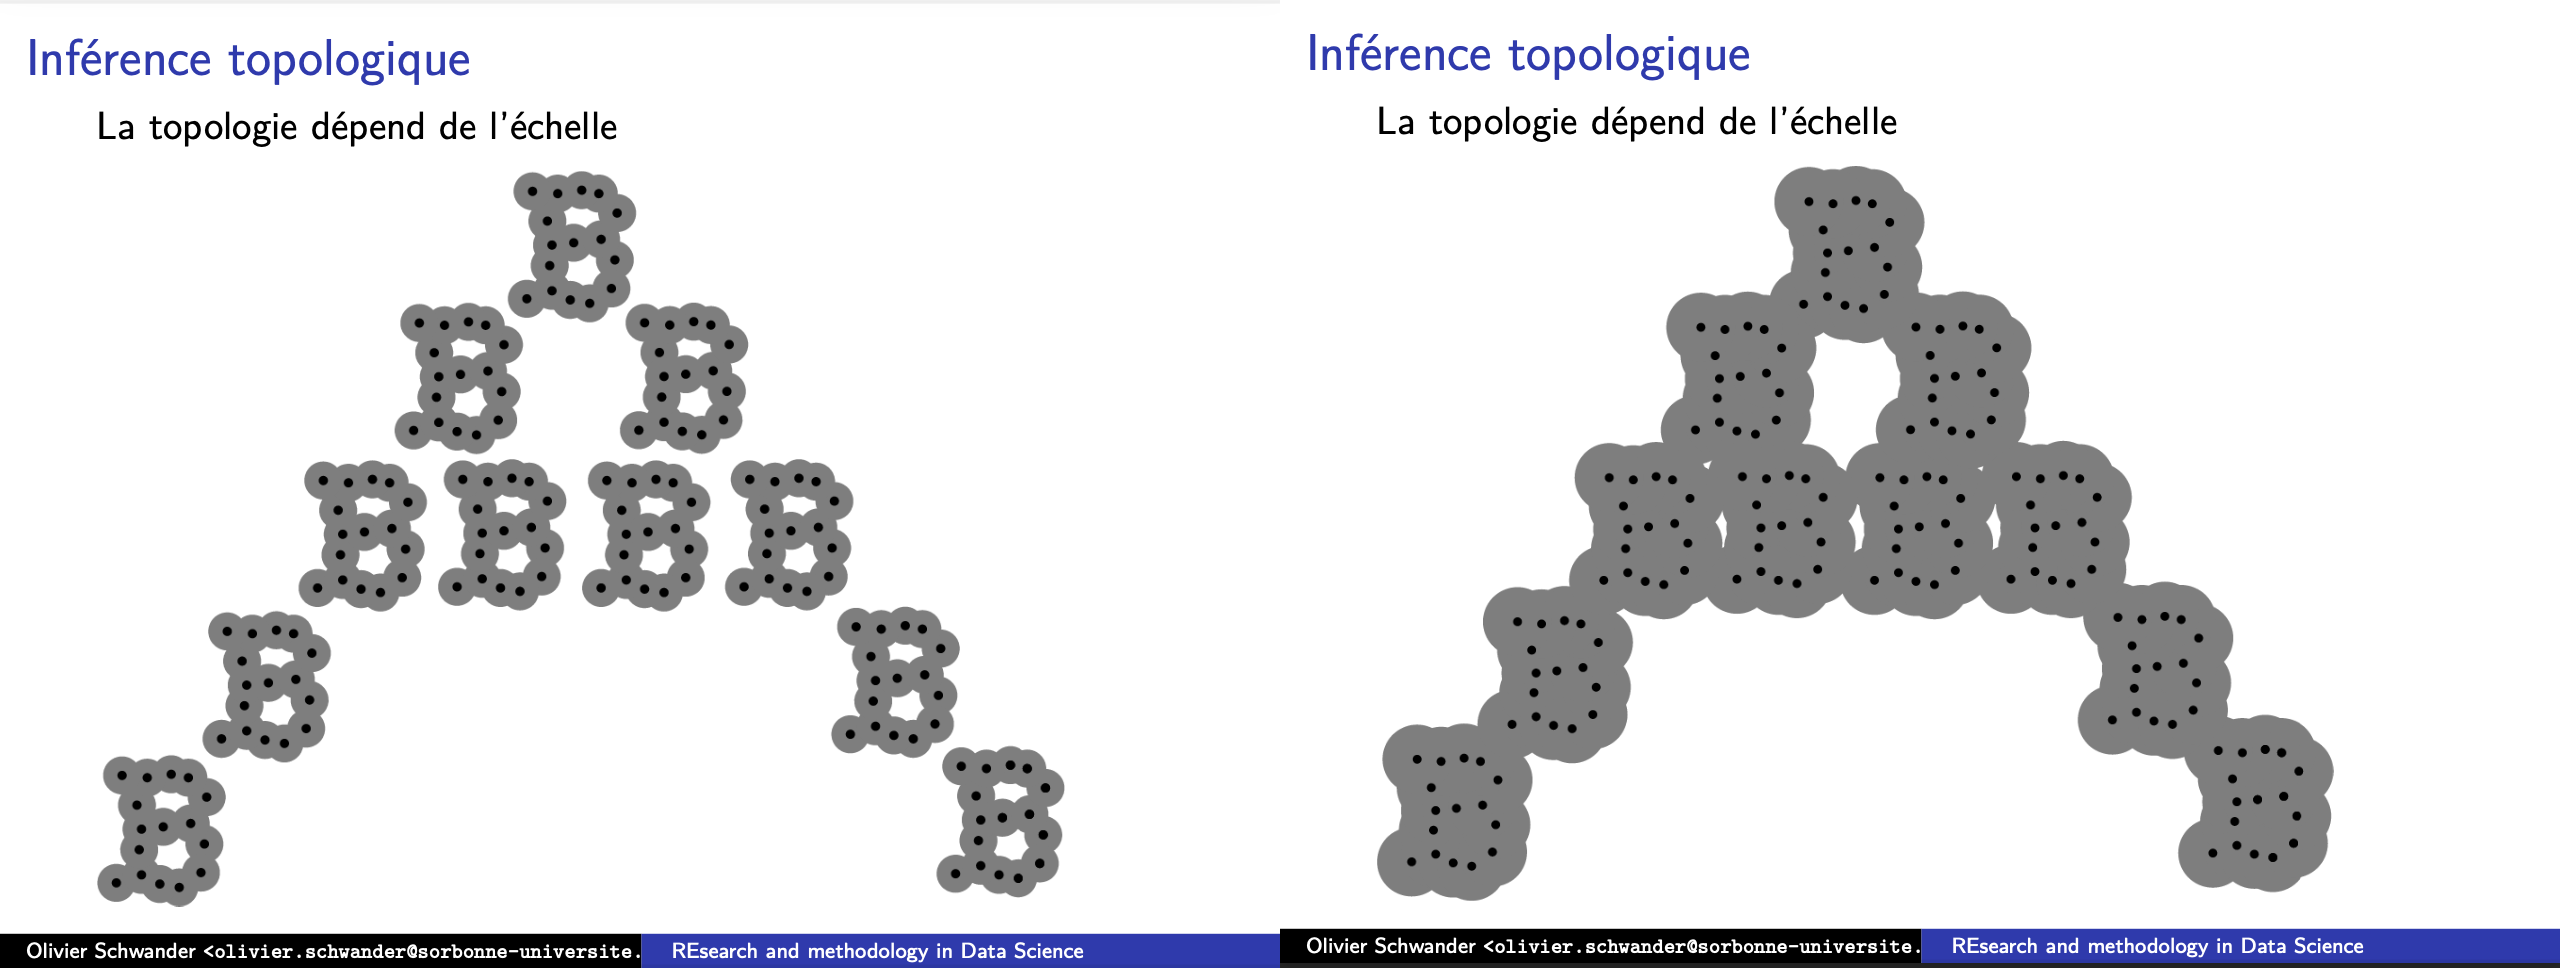
\includegraphics[width=14cm]{scale.png}
\caption{Structure changes with scale}
\label{fig:scale}
\end{figure}

\begin{figure}[H]
  \centering
  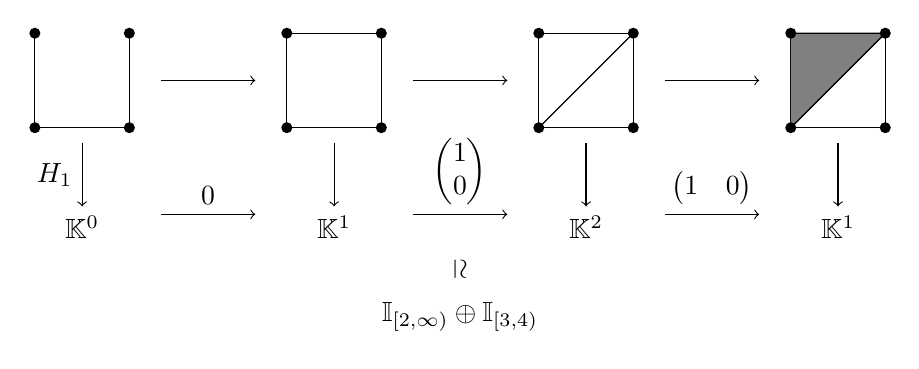
\begin{tikzpicture}[scale=0.4]

  \coordinate (v1) at (0,0);
  \coordinate (v2) at (0,3);
  \coordinate (v3) at (3,0);
  \coordinate (v4) at (3,3);
  \draw (v1) -- (v2);
  \draw (v3) -- (v4);
  \draw (v1) -- (v3);

  \coordinate (w1) at (8+0,0);
  \coordinate (w2) at (8+0,3);
  \coordinate (w3) at (8+3,0);
  \coordinate (w4) at (8+3,3);
  \draw (w1) -- (w2);
  \draw (w3) -- (w4);
  \draw (w1) -- (w3);
  \draw (w2) -- (w4);
  \draw[->] (4,1.5) -- (7,1.5);

  \coordinate (u1) at (16+0,0);
  \coordinate (u2) at (16+0,3);
  \coordinate (u3) at (16+3,0);
  \coordinate (u4) at (16+3,3);
  \draw (u1) -- (u2);
  \draw (u3) -- (u4);
  \draw (u1) -- (u3);
  \draw (u2) -- (u4);
  \draw (u1) -- (u4);
  \draw[->] (12,1.5) -- (15,1.5);

  \coordinate (uu1) at (24+0,0);
  \coordinate (uu2) at (24+0,3);
  \coordinate (uu3) at (24+3,0);
  \coordinate (uu4) at (24+3,3);
  \draw (uu1) -- (uu2);
  \draw (uu3) -- (uu4);
  \draw (uu1) -- (uu3);
  \draw (uu2) -- (uu4);
  \draw (uu1) -- (uu4);
  \filldraw[fill=gray] (uu1) -- (uu4) -- (uu2);
  \draw[->] (20,1.5) -- (23,1.5);

  \foreach \vertex in {v1,v2,v3,v4,w1,w2,w3,w4,
  u1,u2,u3,u4,
  uu1,uu2,uu3,uu4}
    \fill (\vertex) circle (5pt);

  \coordinate (d) at (1.5,-0.5);
  \draw[->] ($(v1)+(d)$) -- node[left] {$H_1$} ++(0,-2) node[below] {$\K^0$};
  \draw[->] ($(w1)+(d)$) -- ++(0,-2) node[below] {$\K^1$};
  \draw[->] ($(u1)+(d)$) -- ++(0,-2) node[below] {$\K^2$};
  \draw[->] ($(uu1)+(d)$) -- ++(0,-2) node[below] {$\K^1$};

  \draw[->] (4, -2.75) -- node[above] {$0$}++(3,0);
  \draw[->] (12,-2.75) -- node[above] {$\begin{pmatrix}1\\0 \end{pmatrix}$}++(3,0);
  \draw[->] (20,-2.75) -- node[above] {$\begin{pmatrix}1 & 0 \end{pmatrix}$}++(3,0);
  
  \node at (13.5,-4.5) {\rotatebox{270}{$\simeq$}};
  \node at (13.5,-6) {$\I_{[2, \infty)} \oplus \I_{[3, 4)}$};

\end{tikzpicture}
  \caption{Filtration gives persistence module gives decomposition gives barcodes}
  \label{fig:tda_diagram}
  \end{figure}

\paragraph{Similarity Filtration with Time Skeleton (SIFTS) \cite{Zhu_2013}}

As in KNN we choose an embedding and a
distance. Then we construct a filtration (a sequence of inclusions
of simplical complexes) of Rips Complexes.

\begin{definition}[Rips complex]
  Given a symmetric matrix $M \in M_n(R^+)$, we define a filtration of Rips complexes
  $$
  (V_d := \{A \subset \llbracket 1, n\rrbracket :
  \forall 1\le i<j\le n, M_{i, j} \le d\})_{d\ge 0}
  $$
\end{definition}
\RM A simplex appears when the last appearance of the its faces happens.

Given an essay, we split it to sentences in order. We embed each sentence by tf-idf.
Then we construct our matrix $M$ by setting $M_{i, j} = 1-\cos(\theta_{i,j})~\text{(the cosine distance)}$
where $\theta_{i, j}$ is the angle between the vectors embedded by the ith and jth sentences.
Then we set $M_{i, i+1} = 0$ (this is where the ``time skeleton'' come from, the reason is
to preserve the order of the essay). We obtain then
a filtration of Rips complexes.
In the filtration, what all this means is that,
at index 0, we will have a skeleton from the first sentence to the last sentence,
then we add simplexes with closer points then those with further points.

After having the filtration, we count the ``number of holes'' of dimension 2
that appears in the filtration (this is formally the \textbf{number of
barcodes} of dimension 2 after we decompose the persistence module
induced by the filtration c.f.\ Figure~\ref{fig:tda_diagram}).
Note that if we just count the number of holes at each index for the filtration,
it would be trivial and not useful, we have to be able to identity the holes
throughout the filtration so that we don't count a hole twice.

We hope to show that this number of holes reflects the quality of arguments of an essay.

\paragraph{Experiment on a real set of data}

data source (more precisely, the essay set 2, which is discoursive) :
\url{https://www.kaggle.com/datasets/thevirusx3/automated-essay-scoring-dataset/code?select=training_set_rel3.tsv}

\begin{figure}[H]
\begin{minipage}{0.49\linewidth}
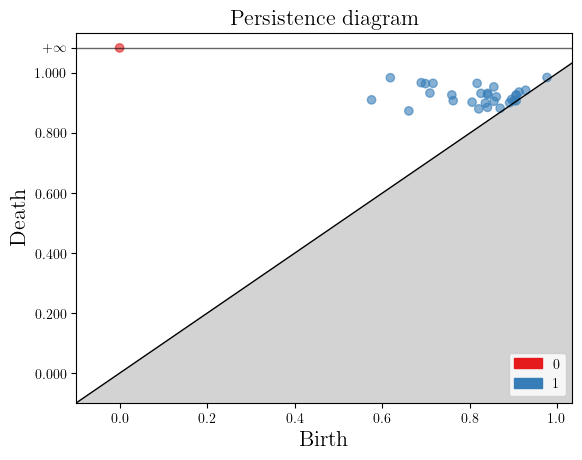
\includegraphics[width=8cm]{pdessay.png}
\end{minipage}
\begin{minipage}{0.49\linewidth}
In @DATE1's world, there are many things found offensive.  Everyone has their own opinion on what is offensive and what is not. Many parents are becoming upset because they think their children are viewing things that they should not.  Other people are upset because they think the libraries are offending their culture or way of life.  This is even taken to the extreme where people want censhorship on libraries to avoid this, which is wrong.     Some people are becoming concerned about the materials in libraries.  They find these things to be offensive.  Everyone is entitled to their own opinion, but there really is nothing anyone can do if someone is offended.  The world is a public place and everywhere we go, something might be found offensive.  The library is a place for study.  It is never intended to offend someone, or bring bad to the world.  It is simply a place to inform, and if someone is offended by what they see, they should stay away from the library.     I have been to the library many times, none of which have I ever seen anything offensive.  Everything I have ever witnessed at the library is for learning and research...
\end{minipage}
\caption{The persistence diagram of an essay of grade 4/6 : A point $(x, y)$ in this diagram corresponds to
a interval module of extremities $x, y$ in the homology of certain degree.
We have many blue points meaning many holes in dim 1, one red point meaning
one homology group of dim 1
}
\label{fig:pd}
\end{figure}

\begin{figure}[H]
% \centering
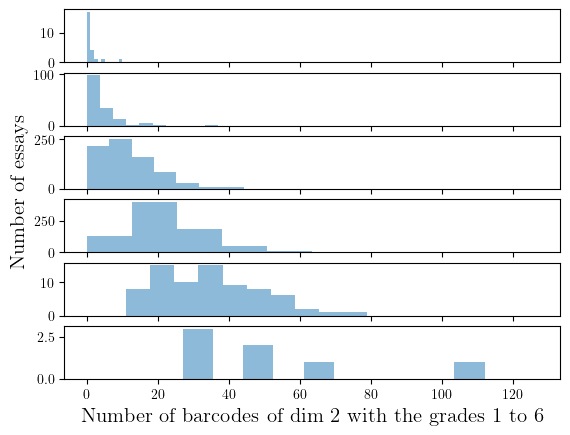
\includegraphics[width=8cm]{gradesh1.png}
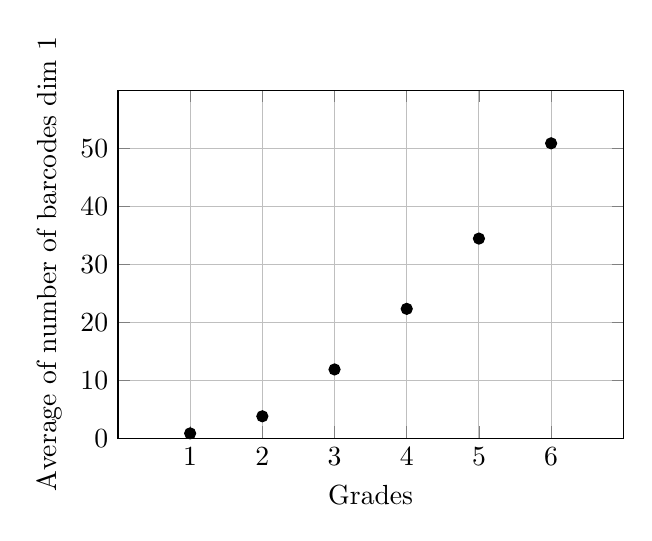
\begin{tikzpicture}
  \begin{axis}[
    xlabel={Grades},
    ylabel={Average of number of barcodes dim 1},
    grid=both,
    xmin=0,
    ymin=0,
    xmax=7,
    ymax=60,
    xtick={1,2,3,4,5,6},
    ytick={0,10,20,30,40,50},
    width=8cm,
    height=6cm,
    ]
    
    \addplot[only marks, mark=*, mark size=2pt] coordinates {
        (1, 0.8333333333333334)
        (2, 3.7777777777777777)
        (3, 11.857142857142858)
        (4, 22.308483290488432)
        (5, 34.42666666666667)
        (6, 50.857142857142854)
    };
  \end{axis}
\end{tikzpicture}
\caption{Number of barcodes increases as grade increases}
\label{fig:ds}
\end{figure}

Those are some discoursive essays on the topic of offense/censorship. We first inspect
an essay with grade 4/6 as an example Figure~\ref{fig:pd}. Then we show
the average of number of holes for each grade (1-6)
as well as the average of number of barcodes for each grade (Figure~\ref{fig:ds}).
We find that number of holes increases as grade increases.

But there are other factors other than the richness of structure of the essay that may affect
the number of holes, like the number of sentences (if we have more points in the set
we will have more chances to form holes) or the number of words.

\begin{figure}[H]
  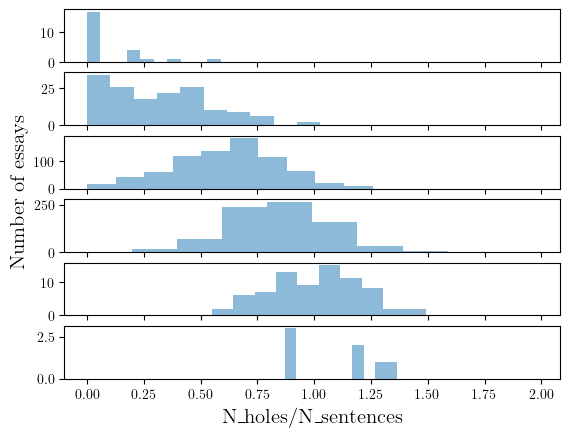
\includegraphics[width=8cm]{gradesah1s.png}
  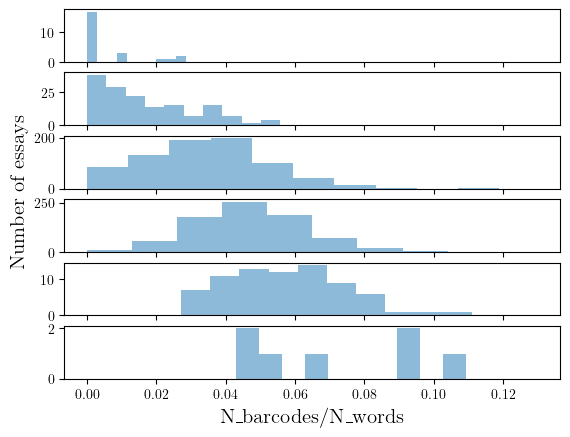
\includegraphics[width=8cm]{gradesah1w.png}
  \caption{The average of barcodes each sentence/word increases as grade increases}
  \label{fig:ads}
\end{figure}

First, let's try to eliminate the effect of number of sentences/number of words
by dividing it (Figure~\ref{fig:ads}). So as we expected, it still shows an simulated
increase of number of barcodes and grade. But even now we may suspect that,
maybe the number of barcodes is just the number of sentences squared. To show that
this is not the case, we fix the number of sentences/the number of words in a range
and inspect the number of barcodes.

\begin{figure}{h}
  \begin{minipage}[t]{0.33\textwidth}
  \centering
  \begin{tabular}{|c|p{2.5cm}|}
  \hline
  \multicolumn{2}{|c|}{Number of Sentences 30-35} \\
  \hline
  Grade & Average of Number of Barcodes \\
  \hline
  3 & 30.75 \\
  4 & 32.0 \\
  5 & 33.06 \\
  6 & 28.33 \\
  \hline
  \end{tabular}
  \end{minipage}%
  \begin{minipage}[t]{0.33\textwidth}
  \centering
  \begin{tabular}{|c|p{2.5cm}|}
  \hline
  \multicolumn{2}{|c|}{Number of Sentences 40-45} \\
  \hline
  Grade & Average of Number of Barcodes \\
  \hline
  3 & 40.0 \\
  4 & 45.96 \\
  5 & 49.45 \\
  6 & 52.0 \\
  \hline
  \end{tabular}
  \end{minipage}%
  \begin{minipage}[t]{0.33\textwidth}
  \centering
  \begin{tabular}{|c|p{2.5cm}|}
  \hline
  \multicolumn{2}{|c|}{Number of Sentences 50-55} \\
  \hline
  Grade & Average of Number of Barcodes \\
  \hline
  3 & 63.0 \\
  4 & 50.0 \\
  5 & 79.0 \\
  \hline
  \end{tabular}
  \end{minipage}

  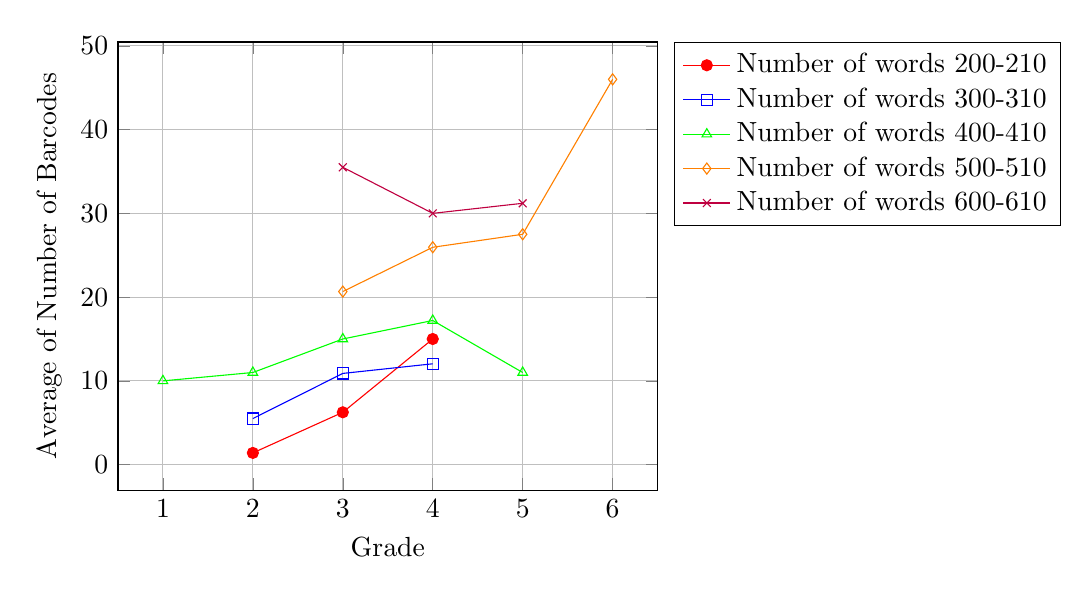
\begin{tikzpicture}
    \begin{axis}[
      xlabel={Grade},
      ylabel={Average of Number of Barcodes},
      legend pos=outer north east,
      grid=both,
    ]
    
    % Number of words 200-210
    \addplot[color=red,mark=*] coordinates {
      (2, 1.4)
      (3, 6.25)
      (4, 15.0)
    };
    
    % Number of words 300-310
    \addplot[color=blue,mark=square] coordinates {
      (2, 5.5)
      (3, 10.89)
      (4, 12.04)
    };
    
    % Number of words 400-410
    \addplot[color=green,mark=triangle] coordinates {
      (1, 10.0)
      (2, 11.0)
      (3, 15.0)
      (4, 17.21)
      (5, 11.0)
    };
    
    % Number of words 500-510
    \addplot[color=orange,mark=diamond] coordinates {
      (3, 20.66)
      (4, 25.95)
      (5, 27.5)
      (6, 46.0)
    };
    
    % Number of words 600-610
    \addplot[color=purple,mark=x] coordinates {
      (3, 35.5)
      (4, 30.0)
      (5, 31.2)
    };
    
    \legend{
      Number of words 200-210,
      Number of words 300-310,
      Number of words 400-410,
      Number of words 500-510,
      Number of words 600-610
    }
    
    \end{axis}
    \end{tikzpicture}

  \caption{Grades and averages of number of holes within fixed sentence/word number ranges}
  \label{tab:gar}
\end{figure}

Seeing Figure~\ref{tab:gar}, we indeed observe and confirm the correlation of increase
that we conjectured. However, the correlation is not absolute as we can constate.
This is because we don't have enough data (for almost all contradictory data
we have selected only one essay of that grade in that range) and other factors than the argument
do affect the grade too (barcodes only show the structure of an essay, for which we
chose to do the tests on discoursive essays). Typically, the wording
of essays of grade 3 but with 30-40 barcodes is bad and repetitive, which is
probably the reason why they are graded not high.

In conclusion, while in Figure~\ref{fig:ads} we have enough essays as example with the default that
the method(division) is not solidly convincing, and in Figure~\ref{tab:gar} we don't
have enough essays for each range though the method is solid, with them combined,
we are confident that the number of barcodes of dim 1 is a good mesure of the quality of
argument structure of an essay.

\paragraph{Further} We may provision studying the identification of type
of arguments (or in previous case, type of comments) by exploiting persistent homology structure,
trying higher dimensional persistent homology etc. But our journey ends here.

\subsection{Theoretical}
\label{theoretical}

This content is a synthesis of this course\cite{INF556} and other
information on the internet.

\paragraph{Motivation} Given a point set, find the underlying (homological) structures of
the data. First, let's consider a topological space, how do we determine
the homology structure of the space in a computational way.

\begin{definition}[$p$-simplex ($p\in\N$)]
  Let $V$ be some finite set (the vertices).
  A $p$-simplex $\sigma$ is the convex hull of $p+1$
  points $x_0, \ldots, x_p \in V$.
  We denote $\sigma = \conv\{x_0, \ldots, x_p\}$ a subset of $V$.
\end{definition}
\RM In practice, we simplify a topological space to its homology equivalence (thin
triangulation) without
losing the information we want (connected components, holes).

\begin{definition}[Face]
  A face of $\sigma$ is $\conv(S)$ where $S\subset\{x_0,\ldots, x_p\}$
\end{definition}

\begin{definition}[Simplicial complex]
  A simplicial complex $X$ is a finite collection of simplices s.t.
  $$
  \forall \sigma\in X, \forall \tau\subset\sigma, \tau\in X
  $$
\end{definition}

\begin{definition}[Chain space]
  The vectorial space of $k$-chains of a simplicial complex $X$ over a field $\K$ is defined by:
  $$
  C_k(X) := \left\{\sum_{i=1}^{\left|X_k\right|} \alpha_i \sigma_i: \alpha_i \in \mathbb{K}, \sigma_i \in X_k\right\}
  \simeq \K^{|X_k|}
  $$
  where $X_k = \{A\subset X : |A|=k+1\}$ the set of $k$-simplexes in $X$.
\end{definition}
\RM Let's work with $\K = \Z/2\Z$ so that we don't consider orientation.

\begin{definition}[$p$-chain]
  A $p$-chain is a subset of $p$-simplices in a simplicial complex $X$.
\end{definition}

\begin{definition}[Boundary operator]
  $$
  \begin{aligned}
  \partial_k: C_k(X) & \to C_{k-1}(X) \\
  \sigma=\{ v_0, \ldots, v_k \} & \mapsto \sum_{j=0}^k(-1)^j \underbrace{ \{v_0,\ldots,v_k \} \setminus \{v_j\}}_{\in X_{k-1}} \\
  \left(\lambda \sigma+\sigma^{\prime}\right) & \mapsto \lambda \partial_k \sigma+\partial_k \sigma^{\prime} \text{ (linear extension)}
  \end{aligned}
  $$
\end{definition}

\begin{lemma}
  $$
  \forall k, \partial_k \partial_{k+1} = 0
  $$
  \label{lem:pp0}
\end{lemma}

\begin{definition}[$k$-th homology group]
  \begin{itemize}
    \item $k$-cycles : $Z_k:=\Ker(\partial_k)$
    \item $k$-boundaries : $B_k:=\Im(\partial_{k+1})$
  \end{itemize}
  The $k$-th homology group of $X$ for the field $\K$ is the following quotient
  of vector spaces:
  $$
  H_k(X):={Z_k\over B_k}
  $$
  (well defined because of the Lemma~\ref{lem:pp0})
  The $k$-th Betti number $\beta_k = \mathrm{rank}(H_k)$.
\end{definition}
\RM The computational method is by Gauss elimination, we omit it here
because we later introduce a method to calculate barcodes which is more
powerful and uses Gauss elimination too.

Now, we are able to give the homology structure of a given topological space (simplicial complex).
Let's go back to the beginning, initially, we are only given a point set,
we may link the points in the set to form a simplicial complex.
The way in which we link the points change our view of the underlying structure.
The scale matters Figure~\ref{fig:scale}.


\begin{definition}[Filtration]
  A filtration over $T$ is a family $\F = (F_t)_{t\in T}$ of increasing topological spaces:
  $$
  \forall t, t^{\prime} \in T, t \leqslant t^{\prime} \Rightarrow F_t \subset F_{t^{\prime}}
  $$
\end{definition}

\begin{definition}[Persistence module]
  Let $\mathbb{K}$ be a given field. A persistence module over $T \subset \mathbb{R}$ is a family $\mathbb{V}=\left(V_t\right)_{t \in T}$ of $\mathbb{K}$-vector spaces
  endowed with linear application $v_t^{t^{\prime}}: V_t \rightarrow V_{t^{\prime}}$ induced by
  a filtration by being applied $H_k$ (e.g.\ Figure~\ref{fig:tda_diagram}).

  $\I_{[l, r)}$(or $\I_{[l, r]}$ etc.) is an interval module with $T = [l, r)$,
  $(V_t)_t = (\K)_t$, $(v^{t'}_t) = (\id)$.
\end{definition}

\begin{theorem}[Decomposition theorem]
  A persistence module $\mathbb{V}$ can be decomposed as a direct sum of interval module
  in the following case (sufficient, not necessary):
  \begin{itemize}
    \item If $T$ is finite. [Gabriel, 72]
    \item When all the vector spaces $V_t$ are finite-dimensional. [Crowley-Boevey, 2012]
  \end{itemize}
  Furthermore, when it exists, the decomposition is unique (up to isomorphism and ordering of terms).
  See an example at Figure~\ref{fig:tda_diagram}
\end{theorem}

\RM Intuitively, the way to decompose is beginning from where a cycle occurs
and following the linear map until it diminishes and concluding an interval module;
the multiset of pairs of extremities of the intervals obtained by decomposition is called the \textbf{barcodes}
or the persistence diagram; to compute the decomposition, we do Gauss elimination (explained in the following).

\subsubsection{Algorithm to calculate the persistence diagram}

\paragraph{Input} A simplicial filtration, that is a filtration over a simplicial complex $K$ which verifies:
\begin{itemize}
  \item $T=\{1, \ldots, m\}$ (finite, so we have a decomposable filtration).
  \item $K_1=\{\sigma_1\}, K_m = K$
  \item $\forall t \in T, K_t$ is a simplicial complex,
  which is a sub-complex of $K_{t+1}$.
  \item We only add one simplex at each step,
  that is $K_{t+1} \backslash K_t=$ $\left\{\sigma_{t+1}\right\}$.
\end{itemize}

\begin{algorithm}
  \caption{Compute the barcodes corresponding to a simplicial filtration}
  \begin{algorithmic}
  \State M := the matrix of boundray operator $\partial$ =: $(c_0, \ldots, c_m)$
  \State $\mathrm{low}(j):=\left\{\begin{array}{l}\max \left\{i \mid M_{i j} \neq 0\right\} \\ 0 \text { if } M_{i j}=0 \text { for all } i\end{array}\right.$
  \For{$j = 1\ldots m$}
  \While{$\exists i<j$ s.t. $\mathrm{low}(i)=\mathrm{low}(j) \neq 0$}
  \State $c_j \gets c_j+c_i$ (Still working with $\K = \Z/2\Z$)
  \EndWhile
  \EndFor
  \State Barcodes are $\{(i, \max\{j \mid \mathrm{low}(j)=i\}) \mid c_i = 0\}$
  (1. This is a multiset 2. $\max$ return $\infty$ if empty 3. the set where we take max is of size at most 1)
  \end{algorithmic}
\end{algorithm}

\begin{proof}[Proof of validity]
Each $c_i = 0$ means the birth of a cycle (one plus for the dimension of the kernel).
Each $c_i \not= 0$ trivialize a cycle (one plus for the dimension of the image).
It remains to show that the pairing is right.

Consider a $c_j \not= 0$, $c_j = e_{l_1} + \cdots + e_{l_k}~(0\le l_1 < \cdots < l_k < j)$.
Note that $\partial_d (\sigma_{l_1} + \cdots + \sigma_{l_k}) = 0$ (Lemma~\ref{lem:pp0}).
So $c_{l_k} = 0$. A posteriori, we can say that $(\sigma_{l_1} + \cdots + \sigma_{l_k})$
this cycle is created at $l_k$ as in a base of $\Ker \partial_d$ (we construct
such base a posteriori in this way).

So the pairing is right.

\end{proof}

\subsubsection{Stability theorem}

\newcommand{\Dg}{\mathrm{Dg}}

\begin{definition}[Homological critical value]
  Let $X$ be a topological space and $f : X \to \R$ a function.
  A homological critical value of $f$ is a real number $b$ for which
  there exists an integer $k$ such that $\forall \epsilon > 0, $
  $H_k(f^{-1}(-\infty, b-\epsilon]) \to H_k(f^{-1}(-\infty, b])$ is not
  an isomorphism.
\end{definition}

\begin{definition}[Tame]
  A function $f : X \to \R$ is tame if it has a finite number of homological
  critical values and the homological groups $H_k(f^{-1}(-\infty, a])$ are finite-dimensional
  for all $k\in\Z$ and $a\in\R$.
\end{definition}
\RM So that the first condition of the decomposition theorem is satisfied
and we have a finite number of barcodes.

\begin{theorem}[Stability Theorem]
  For any two tame functions $f, g : X \to \R$
  $$
  d_\infty(\Dg~f, \Dg~g) \le \|f-g\|_\infty
  $$
  where
  $$
  d_\infty(\Dg~f, \Dg~g) =
  \inf_{m : \Dg(f)\sqcup \Delta \stackrel{\sim}{\to} \Dg(g)\sqcup \Delta}
  ~~
  \sup_{t\in \Dg(f)\sqcup \Delta} \|t-m(t)\|_\infty
  $$
  and $\Dg$ denotes the persistence diagram.
\end{theorem}

\begin{figure}
\centering
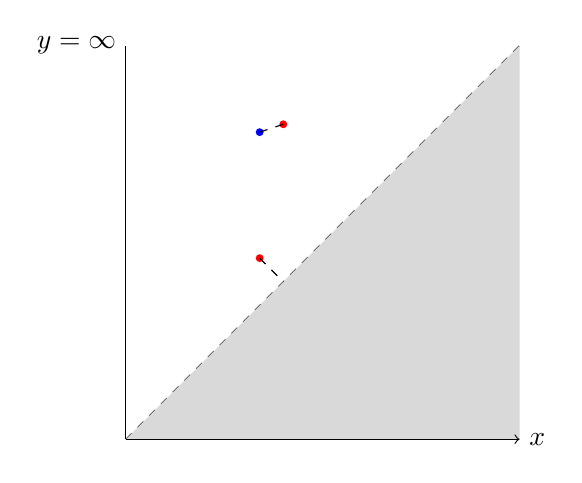
\begin{tikzpicture}
  \draw[dashed] (0, 0) -- (5, 5);
  \fill[gray!30] (0, 0) -- (5, 5) -- (5, 0) -- cycle;
  \draw[->] (0, 0) -- (5, 0) node[right] {$x$};
  \draw[-] (0, 0) -- (0, 5) node[left] {$y=\infty$};
  \fill[red] (1.7, 2.3) circle (0.05);
  \fill[red] (2, 4) circle (0.05);
  \fill[blue] (1.7, 3.9) circle (0.05);

  \draw[dashed] (2, 4) -- (1.7, 3.9);
  \draw[dashed] (1.7, 2.3) -- (2, 2);
\end{tikzpicture}
\caption{Barcodes matching on a persistence diagram}
\label{fig:persistence diagram domaine}
\end{figure}

\begin{proof}
  Let $f, g : X \to \R$ be 2 tame functions. We denote $\varepsilon = \|f-g\|_\infty$.
  We pose $F_t = f^{-1}((-\infty, t]), G_t = g^{-1}((-\infty, t])~(t\in \R)$.

  Key observation: $\left\{F_t\right\}_{t \in \mathbb{R}}$ and $\left\{G_t\right\}_{t \in \mathbb{R}}$
  are $\varepsilon$-interleaved w.r.t. inclusion:\\
  $$
  \forall t \in \mathbb{R}, G_{t-\varepsilon} \subseteq F_t \subseteq G_{t+\varepsilon}
  $$

  We denote
  $F^{2 \varepsilon}=\left\{F_{2 n \varepsilon}\right\}_{n \in \mathbb{Z}}$,
  $G^{2 \varepsilon}=\left\{G_{2(n+1) \varepsilon}\right\}_{n \in \mathbb{Z}}$
  2 discret filtrations.
  $$
  \cdots \subseteq F_0 \subseteq G_{\varepsilon} \subseteq F_{2 \varepsilon} \subseteq \cdots \subseteq G_{(2 n-1) \varepsilon} \subseteq F_{2 n \varepsilon} \subseteq G_{(2 n+1) \varepsilon} \subseteq \cdots
  $$
  We denote another discret filtration $\left\{H_{n \varepsilon}\right\}_{n \in \mathbb{Z}}$, where $H_{n \varepsilon}=\left\{\begin{array}{l}F_{n \varepsilon} \text { if } n \text { is even } \\ G_{n \varepsilon} \text { if } n \text { is odd }\end{array}\right.$

  $$
  d_\infty(f, g) \le d_\infty(f, F) + d_\infty(F, H) + d_\infty(H, G) + d_\infty(G, g)
  \le (2+1+1+2)\varepsilon \le 6\varepsilon
  $$
  (We can optimise it to $\varepsilon$)
  
\end{proof}


\printbibliography

\end{document}
